\documentclass[12pt]{projeto}
\makeatletter
\DeclareRobustCommand{\rm}{\@font@warning{Using old font command \string\rm}\normalfont}
\makeatother
\graphicspath{{figures/}}
% Insira suas informações no arquivo conf.tex
%\usepackage{natbib}
\usepackage[alf]{abntex2cite}
\usepackage[T1]{fontenc}
\usepackage[utf8]{inputenc}
\usepackage[brazil]{babel} % <--- ESSA LINHA É CRUCIAL
\usepackage{aas_macros} 
\usepackage{array} % Certifique-se de que este pacote está no seu preâmbulo.

%\usepackage{fontspec}

%%%%%%%%%% Arquivo de configuração do projeto
%% Insira seus dados e modifique o modelo com suas preferências
%% Comente/descomente linhas para modificar o modelo
%% Aviso! O modelo não segue uma norma específica

%%%%%%%%%%%%%% Informações dos projeto
\tipo{Relatório Final IC - Bolsa PIBIC}
\titulo{Investigando o Efeito Sintético em Modelos Espectrais de Populações Estelares}
\aluno{André Almeida Trovello}
\emailaluno{andretrovello@usp.br}
\orientador{Paula R. T. Coelho}
\emailorientador{pcoelho@usp.br}
\palavraschave{Projeto, Mestrado, Galáxias disco, Populações Estelares}
\data{\today}

%%%%%%%%%%%%%% Pacotes extras
\usepackage{lipsum} % Gera texto dummy
%\usepackage{fullpage} % Uniformiza as margens (1,5 cm) 
\usepackage{xcolor}
\usepackage{geometry}
\geometry{margin=1in}

%%%%%%%%%%%%%% Bibliografia
%% Para referências estilo ABNT tire o comentário de uma das linhas 
%% Manual do pacote de referências: https://www.abntex.net.br/

%\usepackage[num]{abntex2cite}	% Referências numéricas padrão ABNT
%\usepackage[alf]{abntex2cite}  % Referências alfabéticas padrão ABNT

\AtEndDocument{
    \bibliografia{bibtex.bib} % Arquivo com o bibtex
    \estilobibliografico{apalike} % Estilo das referências se não usar ABNT
%% Mais estilos: https://www.overleaf.com/learn/latex/bibtex_bibliography_styles
}

%% Para adicionar backrefs tire o comentário da linha abaixo,
%% backrefs listam as paginas em que uma referência foi citada
%\usepackage[brazilian,hyperpageref]{backref} % Adiciona backrefs

%%%%%%%%%%%%%% Confs
\AtBeginDocument{
    \maketitle % Gera cabeçalho
    \pagestyle{plain} % Efetivamente, insere a numeração
}

%%%%%%%%%%%%%%%% Comandos úteis para matemática
\newcommand{\Z}{\mathbb{Z}}
\newcommand{\Q}{\mathbb{Q}}
\newcommand{\R}{\mathbb{R}}
\newcommand{\trans}{^\intercal}
\newcommand{\pc}[1]{\texttt{\textcolor{magenta}{[#1]}}}

\DeclareMathOperator{\posto}{posto}
\DeclareMathOperator{\capacidade}{cap}
\DeclareMathOperator{\valor}{val}
\DeclareMathOperator{\mdc}{mdc}
\DeclareMathOperator{\adj}{adj}
\DeclareMathOperator{\conv}{conv}
\DeclareMathOperator{\cone}{cone}

\DeclarePairedDelimiter\ceil{\lceil}{\rceil}
\DeclarePairedDelimiter\floor{\lfloor}{\rfloor}

\newtheorem{teorema}{Teorema}
\newtheorem{definicao}{Definição}
\newtheorem{lema}{Lema}
\newtheorem{proposicao}{Proposição}
\newtheorem{corolario}{Corolário}
\newtheorem{fato}{Fato}
\theoremstyle{definition} % Arquivo de configuração

\begin{document}

\begin{abstract}
A determinação de distâncias de aglomerados estelares é crucial para calibrar a escala de distância cósmica, exigindo metodologias que lidem com sistemáticas como a correlação espacial das paralaxes do Gaia DR3. Este trabalho teve como objetivo determinar a distância do aglomerado aberto NGC 1662 utilizando a Inferência Bayesiana hierárquica implementada no código Kalkayotl \cite{olivares_kalkayotl_2020}, avaliando o desempenho de diferentes priors em amostras de dados variadas.

A aplicação demonstrou a robustez do Kalkayotl, mas revelou a sensibilidade do Prior Uniforme à presença de outliers, que se mostrou estatisticamente incompatível, dentro de um intervalo de confiança de \(2\sigma\), com a amostra filtrada ($\text{A}_{\text{cut}}$). Em contraste, os priors Gaussiano, EFF e King apresentaram forte estabilidade e compatibilidade entre as amostras, estabelecendo-se como os mais adequados. O prior Gaussiano, especificamente, forneceu a estimativa final de $\mathbf{411,4^{+2,0}_{-\text{2,0}}} \mathbf{pc}$.

A comparação com a literatura mostrou compatibilidade com o catálogo de Dias et al. (\citeyear{dias_updated_2021}), mas uma incompatibilidade estatística significativa com a distância de alta precisão de Hunt et al. (\citeyear{hunt_improving_2024}), que pode estar atrelada a incertezas subestimadas em seu catálogo Conclui-se que o Kalkayotl é uma ferramenta rigorosa que quantifica a sistemática não corrigida, garantindo que suas incertezas não são subestimadas.
\end{abstract}


\section{Introdução}

A determinação de distâncias é uma questão relevante na astronomia contemporânea. Em especial, a determinação de distâncias de aglomerados estelares se mostra primordial para refinar modelos de formação e evolução estelar, visto que o cálculo dessa grandeza possibilita a conversão de valores aparentes de magnitudes em absolutos, viabilizando a obtenção acurada de parâmetros como idade e massa das estrelas que compõem o aglomerado.

Tradicionalmente, a distância destes aglomerados é calculada pela inversão das paralaxes observadas em seus membros, porém, este método se mostra altamente sujeito a erros aleatórios quando são estudados aglomerados mais distantes, já que nestas ocasiões o erro da paralaxe pode apresentar mesma ordem de grandeza que a própria paralaxe em si.

No contexto deste problema, a missão espacial Gaia \cite{gaia_collaboration_gaia_2016} contribuiu significativamente, fornecendo paralaxes de alta precisão de aglomerados e estrelas. Como toda medida experimental, os dados da Gaia possuem um erro associado, sendo este uma combinação de três fatores principais: erros aleatórios (a incerteza estatística individual de cada fonte), erros sistemáticos (oriundos de fatores como posição, cor e magnitude da estrela, que afetam estrelas próximas no céu de maneira semelhante) e o zero point (um offset de medição sistemático associado ao próprio instrumento Gaia).

Em decorrência da propagação não linear das incertezas da paralaxe, técnicas como a Inferência Bayesiana se mostram como boas alternativas para contornar essa questão, possibilitando calcular a distribuição de probabilidade posterior das distâncias de aglomerados, incorporando a verossimilhança dos dados observados e o conhecimento prévio através dos priors.

Baseado nessa técnica, o código Kalkayotl \cite{olivares_kalkayotl_2020} foi desenvolvido utilizando um framework bayesiano hierárquico para inferir simultaneamente os parâmetros da população e as distâncias individuais das estrelas. Sua abordagem tem a vantagem de tratar as correlações espaciais das paralaxes, provendo estimativas confiáveis de distância e incertezas não subestimadas. 

Este projeto teve como objetivo determinar a distância de um aglomerado aberto por meio do código Kalkayotl 1.0, comparando seus resultados com os publicados na literatura, de forma a visualizar a eficácia do método bayesiano quando confrontado com outras estimativas, e compreender quais priors se adequam melhor ao aglomerado em questão. 

\subsection{Aquisição de Dados e Seleção do Aglomerado}

Os dados de aglomerados foram obtidos a partir do catálogo de Emily L. Hunt \cite{hunt_improving_2024}, que através das medições do Gaia DR3 \cite{vallenari_gaia_2023}, fez um estudo de 6956 aglomerados classificados por trabalhos prévios e verificou a ligação gravitacional de suas estrelas membros, concluindo que apenas 5647 (79\%) deles podem ser considerados abertos, fornecendo também estimativas de distâncias para estes corpos celestes. 

Definido o método e o catálogo analisado, fez-se necessária a determinação de um aglomerado para estudo. Para evitar dificuldades no cálculo da distância, utilizou-se como critério de seleção a proximidade do aglomerado (\(<500\)pc) e a quantidade de estrelas membros (\(>200\)). Dessa forma, foi escolhido o aglomerado NGC 1662 (Figura \ref{fig:NGC1662}), composto por \(384\) estrelas e a (\(404,59 \pm 0,28\)) parsecs de distância, segundo o catálogo de Hunt.
\begin{figure}[ht]
\centering
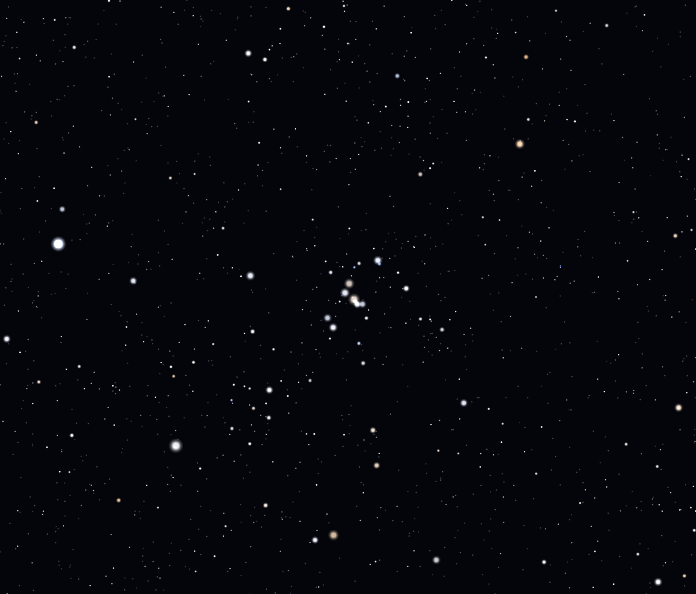
\includegraphics[width= 0.8\textwidth]{NGC_1662.png}
\caption{\label{fig:NGC1662} Aglomerado NGC 1662.}
\end{figure}

\subsection{Revisão da Literatura e Metodologias de Distância}

A estimativa de distância do aglomerado NGC 1662 foi contextualizada e comparada com quatro catálogos notáveis (Tabela \ref{tab:comparativo_distancias_incerteza}) , que ilustram a evolução das metodologias na astrometria galáctica: um catálogo pré-Gaia \cite{dias_new_2002}, dois trabalhos do Gaia DR2 com diferentes abordagens \cite{cantat-gaudin_painting_2020, dias_updated_2021} e um catálogo moderno do Gaia DR3 \cite{hunt_improving_2024}.

Na primeira abordagem, o catálogo DIAS et al., (\citeyear{dias_new_2002})  realizou uma compilação de valores de distância da literatura calculados pelo ajuste da sequência principal fotométrica no Diagrama Cor-Magnitude (CDM) e, no caso de aglomerados próximos, pela inversão da média das paralaxes calculadas pelo satélite Hipparcos \cite{esa_hipparcos_1997}. Para NGC 1662, foi estimada uma distância de \(437\) parsecs, utilizando o método fotométrico. Dado que utilizou de dados de baixa precisão de missões antigas, este método não apresentou incerteza em sua medida.

Com a precisão do Gaia DR2 \cite{gaia_collaboration_gaia_2018}, surgiram métodos mais robustos de determinação de parâmetros, embora com diferentes estratégias para o tratamento de erros. CANTAT-GAUDIN et al., (\citeyear{cantat-gaudin_painting_2020}) utiliza de um modelo de Inferência Bayesiana Hierárquica para inferir a distribuição de probabilidade das paralaxes dos membros de aglomerados, de onde a distância final é obtida por meio da mediana da distribuição de probabilidade \textit{a posteriori}. Embora tenha sido validado, as incertezas finais deste método não foram fornecidas no catálogo, limitando a avaliação de confiabilidade do valor de \(428\) parsecs obtido para NGC 1662.

Por sua vez, \cite{dias_updated_2021} realizou o cálculo de distâncias por meio do ajuste de isócronas (\textit{isochrone fitting}) ao CDM, empregando o algoritmo de entropia cruzada para determinar parâmetros como a distância, idade, extinção e metalicidade. O método incluiu a aplicação de priors e utilizou reamostragem Monte-Carlo (\textit{bootstrapping}) para a determinação das incertezas, obtendo assim um valor de (\(410 \pm 3\)) parsecs para NGC 1662.

Com o advento do Gaia DR3, o aumento na precisão astrométrica permitiu a HUNT; REFFERT,.(\citeyear{hunt_improving_2024}) calcular distâncias novamente por ajuste de isócronas ao CDM. Entretanto, o método foi aprimorado com um estudo estatístico que visa o máximo rigor. A identificação de membros do algomerado é feita pelo algoritmo HDBSCAN (Hierarchical Density-Based Spatial Clustering of Applications with Noise - CAMPELLO; MOULAVI; SAN-
DER \citeyear{campello_density-based_2013}), e a distância final é o resultado de um processo de inferência probabilística de parâmetros. Por ser um método estatístico avançado e de natureza bayesiana em seus resultados, o catálogo fornece a distância como a mediana (50º percentil) da distribuição de probabilidade, acompanhada dos limites do intervalo de confiança (16º e 84º percentis), resultando em nosso último valor de comparação para NGC 1662 de (\(404,60 \pm  0,28\)) parsecs. 


\begin{table}[ht]
    \centering
    \caption{Comparativo das estimativas de distância para NGC 1662 e suas incertezas (quando calculadas).}
    \label{tab:comparativo_distancias_incerteza}
    % Redefinindo o ambiente tabular para usar alinhamento vertical 'm'
    % Adicionamos '\renewcommand{\arraystretch}{1.5}' para um espaço extra uniforme
    \renewcommand{\arraystretch}{1.3} % Aumenta o espaçamento padrão
    \begin{tabular}{|>{\centering}m{5cm}|>{\centering\arraybackslash}m{4cm}|}
        \hline
        \textbf{Autor (Ano)} & \textbf{Distância ($d$) [pc]} \\
        \hline
        Hunt et al. (2024) & $404,60^{+0,28}_{-\text{0,28}}$ \\
        \hline
        Dias et al. (2021) &  $410^{+3}_{-\text{3}}$ \\
        \hline
        Cantat-Gaudin et al. (2020) & $428$ \\
        \hline
        Dias et al. (2002) & $437$ \\
        \hline
    \end{tabular}
    \renewcommand{\arraystretch}{1.0} % Retorna ao padrão
\end{table}

\subsection{Seleção da Amostra}

O estudo de distância do aglomerado NGC 1662 no Kalkayotl foi feito com duas amostras distintas. A primeira, denominada amostra completa (\(A_{full}\)), incluiu todas as 384 estrelas fornecidas inicialmente pelo catálogo de Hunt. 

Entretanto, para descartar a presença de \textit{outliers} que pudessem enviesar o resultado, realizou-se uma segunda seleção (\(A_{cut}\)), onde foram removidas estrelas que estivessem a uma distância de \(2\sigma\) da mediana do conjunto de dados (Figura \ref{fig:selecao_amostral}). Esta filtragem resultou em uma amostra final de 360 estrelas, que foi então utilizada para o cálculo da distância do aglomerado no Kalkayotl.

\begin{figure}[ht]
\centering
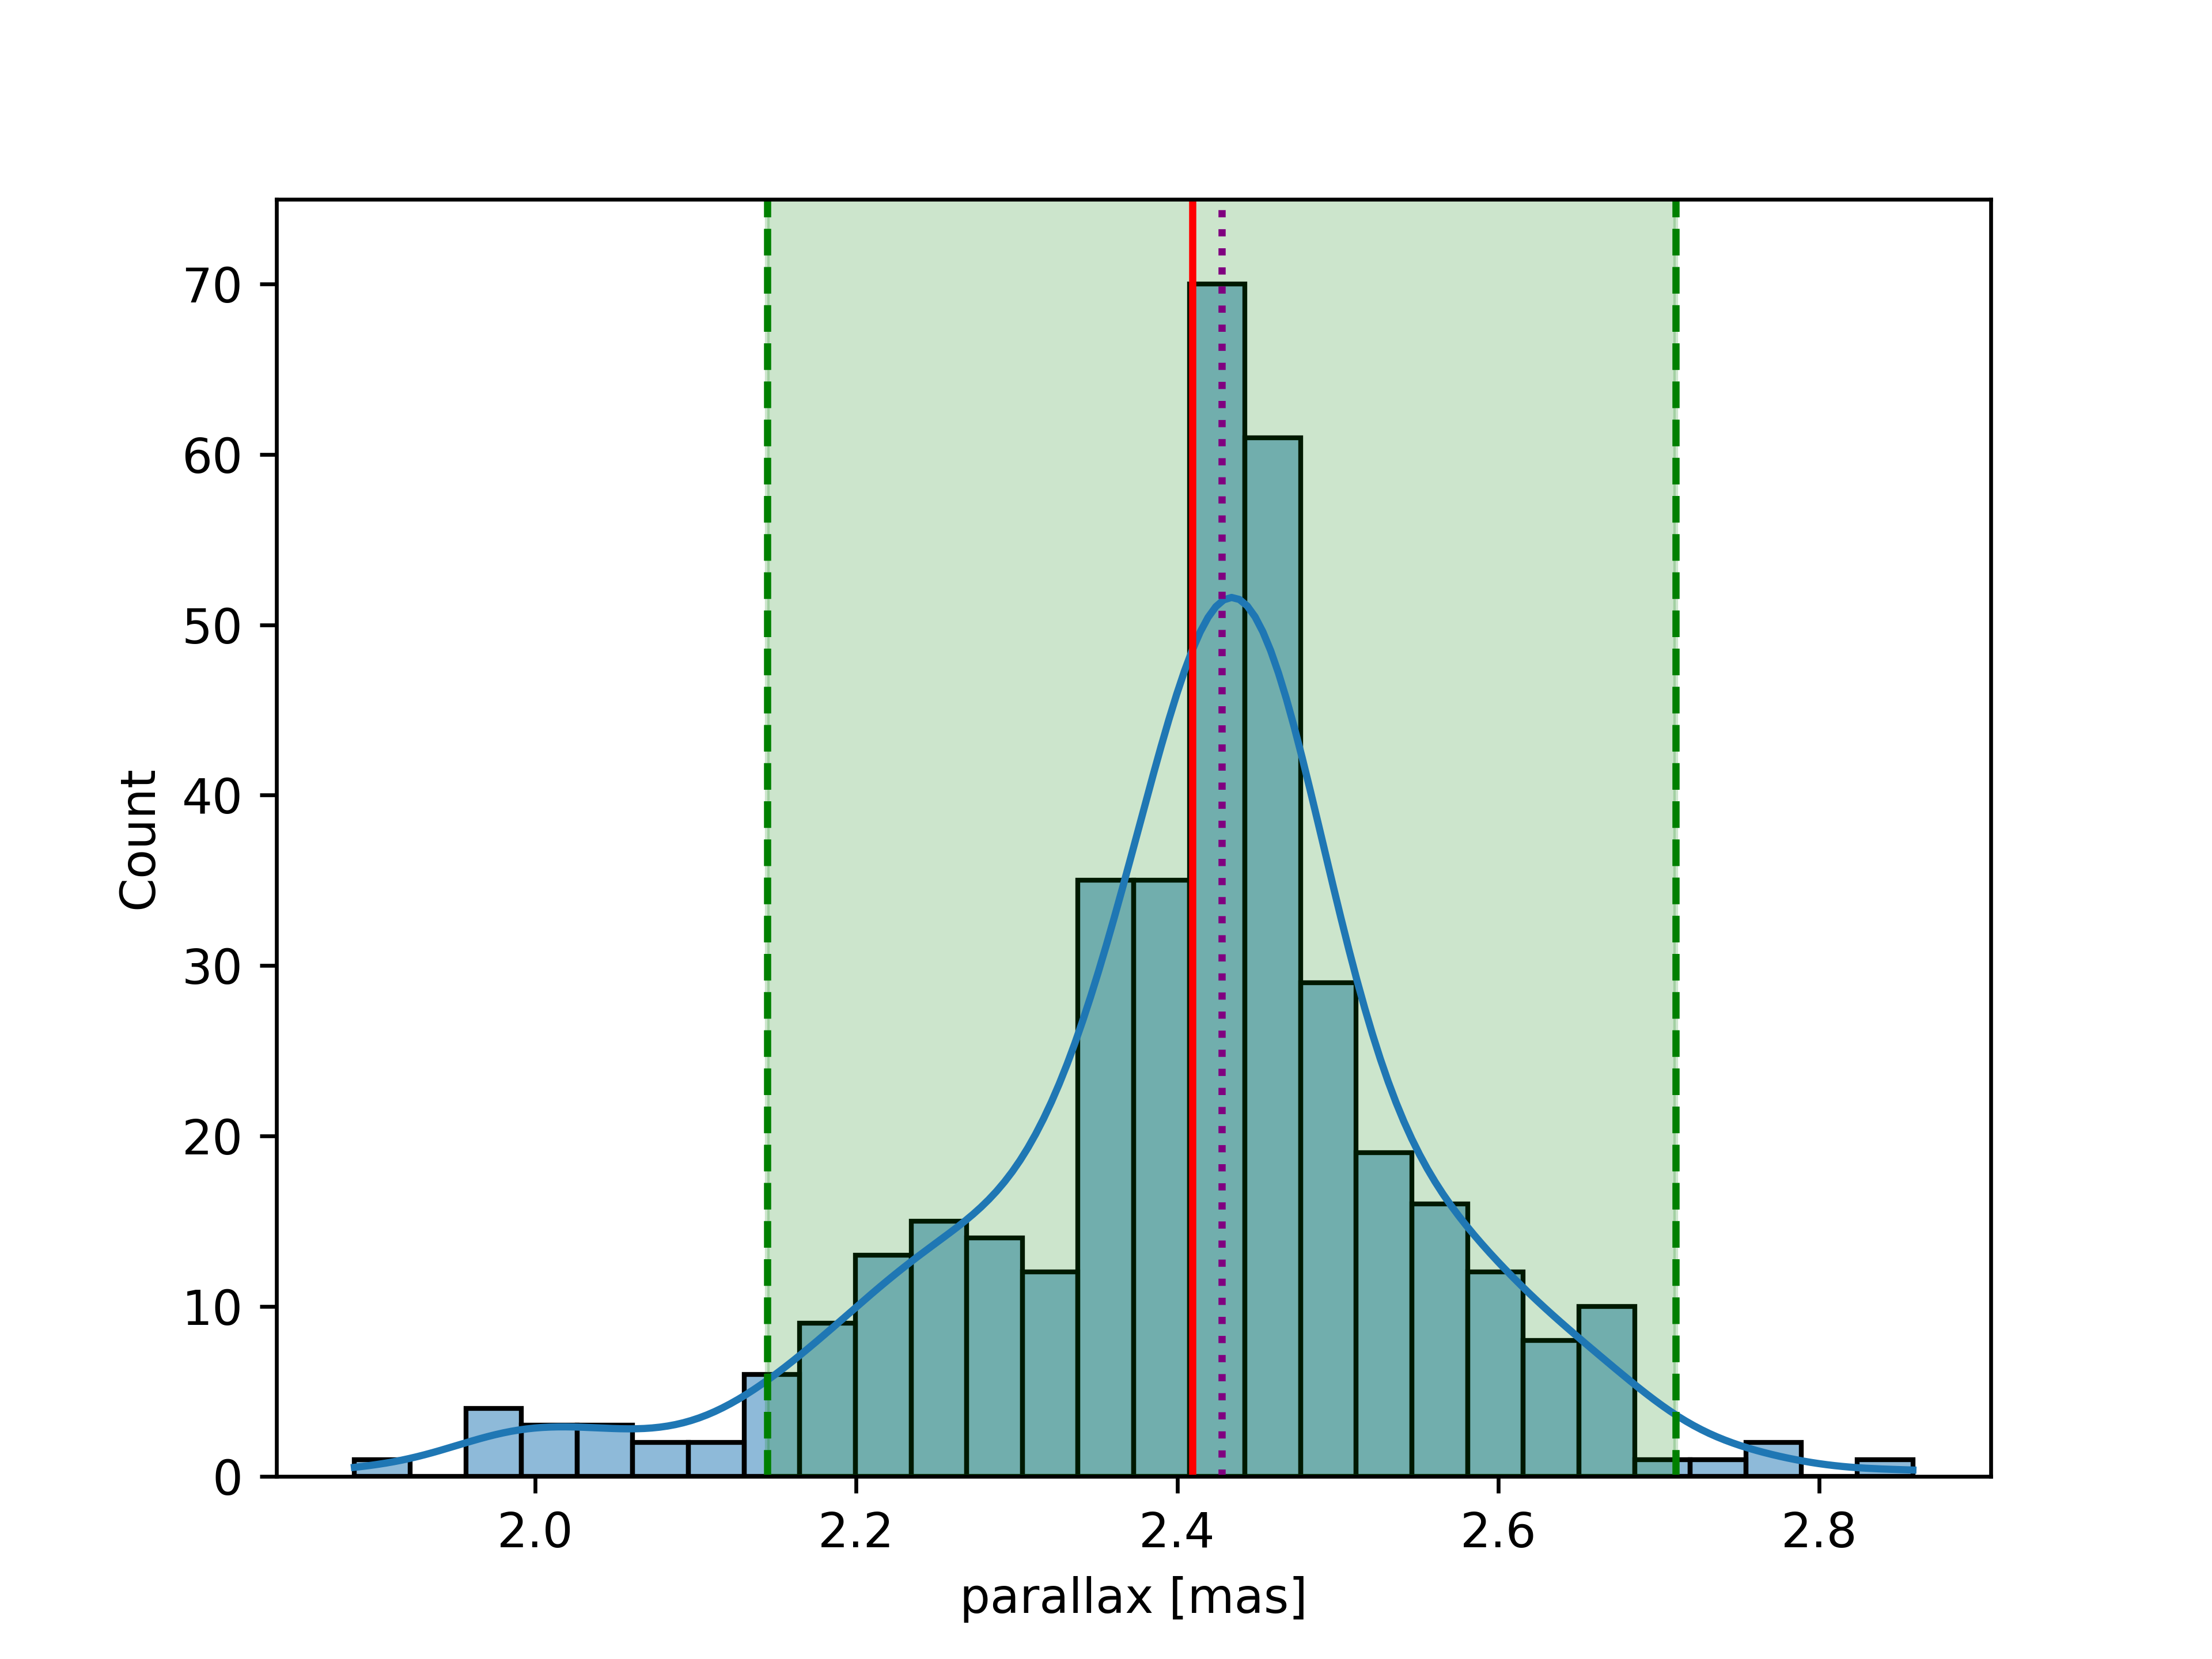
\includegraphics[width= 0.8\textwidth]{NGC1662_parallax.png}
\caption{\label{fig:selecao_amostral} Distribuição dos valores de paralaxe para o aglomerado NGC 1662, bem como a seleção amostral (área verde clara) para \(2\sigma\) (95\%) da mediana (linha pontilhada roxa). Foi escolhida a mediana em detrimento da média (linha vermelha) devido à primeira se aproximar melhor da Estimativa de Densidade de Kernel (KDE, curva verde escura).}
\end{figure}

\subsection{Priors}

A determinação do prior (conhecimento prévio sobre o parâmetro de interesse) é fundamental quando são utilizados métodos de Inferência Bayesiana, visto que garante não apenas a acurácia do modelo, como também a estabilidade da Cadeia MCMC (Markov Chain Monte Carlo), que é o algoritmo central do código Kalkayotl.

A MCMC é uma técnica que permite a obtenção da complexa distribuição de probabilidade posterior dos parâmetros do aglomerado. Ela se baseia na Propriedade de Markov, que estabelece que a probabilidade de a cadeia se mover para o próximo estado depende única e exclusivamente de seu estado atual, e não de sua trajetória anterior. Isso implica que a distribuição de amostragem converge para um estado estacionário, que é a própria distribuição posterior desejada.

No caso do Kalkayotl, a MCMC utiliza de uma amostragem Hamiltonian Monte Carlo (HMC), que utiliza do gradiente da função de verossimilhança para guiar seus próximos passos. Essa técnica possibilita iterações mais informadas, evitando que a cadeia flutue descontroladamente, garantindo a estabilidade do modelo. 

O código Kalkayotl apresenta dois tipos de priors: estatísticos e astrofísicos.

Priors estatísticos são aqueles baseados apenas em distribuições matemáticas simples para a densidade de estrelas do aglomerado. Estes modelos são mais simples, apresentando poucos parâmetros livres, a distãncia do centro do algomerado (\textit{loc}) e seu tamanho ao longo da linha de visada (\textit{scl}). Os três priors estatísticos presentes no código estão descritos abaixo.

\textbf{Uniforme:} prior mais simples, que atribui a mesma densidade de probabilidade para todos os valores no intervalo \([loc-scl,loc+scl]\)  

\textbf{Gaussian:} assume que a distância é uma distribuição normal com média (\textit{loc}) e desvio padrão (\textit{scl}).

\textbf{Gaussan Mixture Model:} GMM é um prior descrito como a combinação linear de \textit{k} distribuições Gaussianas, sendo \(k>0\). Para os estudos deste projeto, \(k=2\).

Por outro lado, priors astrofísicos  são baseados em modelos físicos ou empíricos de estrutura de aglomerados. Apresentam maior complexidade, tendo parâmetros adicionais, além de \textit{loc} e \textit{scl}.

A descrição dos priors astrofísicos presentes no Kalkayotl é feita a seguir.

\textbf{Elson Fall and Freeman:} EFF é um prior que distribui as distâncias da mesma maneira que \cite{elson_structure_1987} distribui a densidade de luminosidade superficial em aglomerados da Grande Nuvem de Magalhães. Além da distância e tamanho do aglomerado, também é adicionado um parâmetro \(\gamma\) que descreve o declive da distribuição em raios grandes.

\textbf{King:} descreve a distribuição de distâncias da mesma forma que \cite{king_structure_1962} descreve a distribuição espacial de aglomerados globulares. Além de \textit{loc} e \textit{scl}, inclui também a máxima extensão do algomerado, por meio do raio de maré (\(r_t\))

\textbf{Exponentially Decreasing Space Density Prior}: introduzido por \cite{bailer-jones_estimating_2015}, o EDSD é um prior galáctico projetado para inferir distâncias a estrelas de campo de toda a Galáxia. Dessa forma, no contexto de um único aglomerado estelar ele não é preciso para inferir distâncias, não sendo portanto utilizado neste projeto. Seu único parâmetro (\textit{scl}) refere-se ao comprimento típico do decaimento exponencial.

\subsection{Definição de Parâmetros}

Para rodar o código Kalkayotl e fazer a análise de inferência, foram definidos alguns parâmetros que garantem a acurácia e a confiabilidade dos resultados, pensando sempre no funcionamento correto da Inferência Bayesiana.

No modelo, reportou-se a \textit{Moda} (\textit{Mode}) da distribuição de probabilidade posterior como a distância central do aglomerado. Essa escolha é estatisticamente mais correta do que usar a média, pois a relação não-linear entre paralaxe e distância cria uma distribuição assimétrica. Com o uso da Moda, garantimos que o valor reportado seja, de fato, a distância mais provável (o  pico da distribuição).

Além disso, \textit{Parametrização Central} foi utilizada no modelo hierárquico. Como o NGC 1662 é um aglomerado próximo ($\sim 400$ pc) e bem populado ($N=384$), o nosso conjunto de dados é altamente restritivo. Neste caso, a parametrização central é a mais eficiente, pois evita as correlações complexas que a parametrização não-central visa resolver em aglomerados mais distantes e com dados mais limitados.

Por fim, definiu-se incerteza dos parâmetros pelo intervalo de confiança de $68\%$, o que equivale a aproximadamente $1\sigma$ em uma distribuição normal, com o objetivo de obter uma boa estimativa de incerteza. Além disso, foi determinado como \(-0,021mas\) o valor de zero point para o Gaia DR3  \cite{groenewegen_parallax_2021}.

Descrito o método, as ferramentas, os dados e o funcionamento do código, seguem, na seção seguinte, os resultados obtidos ao longo deste projeto para o aglomerado aberto NGC 1662.

\section{Resultados e Análise}

Como saída, o Kalkayotl forneceu a densidade de probabilidade das distâncias de estrelas individuais e do aglomerado em si, bem como as iterações das cadeias de Markov em cada caso, retornando resultados como os apresentados na Figura \ref{fig:ex_gaussiano}.

\begin{figure}[ht]
\centering
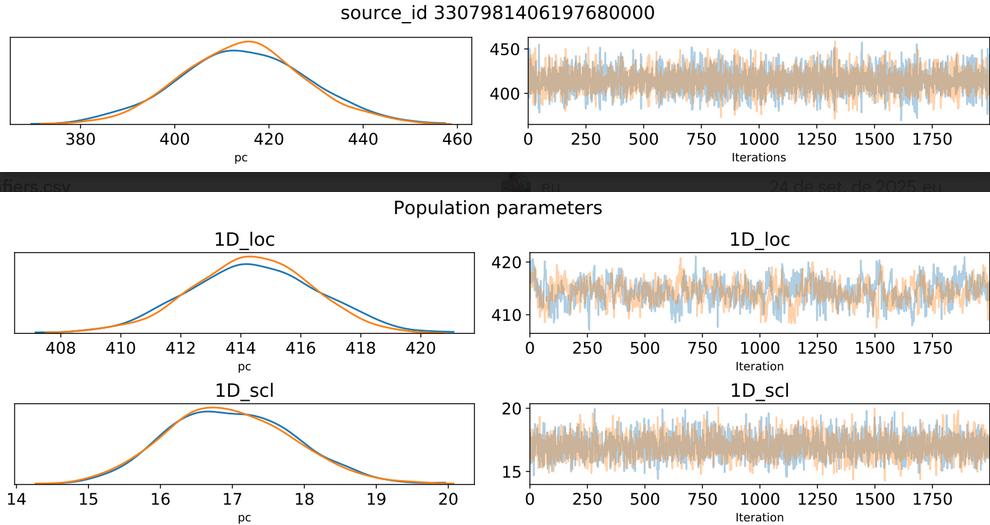
\includegraphics[width= 0.8\textwidth]{gaussian_ngc1662.png}
\caption{\label{fig:ex_gaussiano} Resultados da amostra completa ($A_{full}$) do aglomerado NGC 1662, divididos entre distribuição de probabilidade das distâncias (esquerda) e iterações das cadeias de Markov (direita). A primeira linha apresenta resultados individuais de uma estrela, enquanto as demais referem-se ao aglomerado completo. Prior Gaussiano adotado.}
\end{figure}

Obtidas as curvas apresentadas acima, foi necessária a avaliação dos resultados para estudar a qualidade do prior quando aplicado ao aglomerado em questão. Esse processo foi feito inicialmente pela análise da convergência da Cadeia MCMC. Na maioria dos priors, tanto para \(A_{full}\) quanto para \(A_{cut}\), a convergência foi estável, sem apresentar qualquer tendência de subida ou descida e com um comportsamento muito semelhante entre as cadeias. Entretanto, foram notadas discrepâncias nos resultados do prior GMM da amostra \(A_{full}\) (Figura \ref{fig:gmm_ngc1662full}), onde as cadeias convergiram para valores distintos e não houve sobreposição das distribuições de probabilidade.

\begin{figure}[ht]
\centering
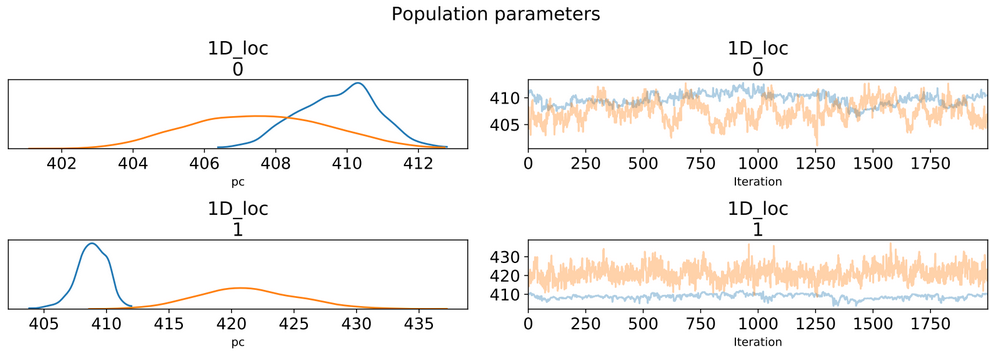
\includegraphics[width= 0.8\textwidth]{gmm_ngc1662full.png}
\caption{\label{fig:gmm_ngc1662full} Resultados dos parâmetros do aglomerado para a amostra \(A_{full}\) para o prior GMM}
\end{figure}

Essa falha de convergência se dá pela própria definição do prior GMM como sendo uma mistura de distribuições Gaussianas, o que implica que um aglomerado que se adapte bem a este modelo apresenta subestruturas em sua composição ou possui amostra muito bem definida. O resultado do GMM permite, portanto, inferir uma morfologia simples para o NGC 1662, que não possui as subestruturas necessárias para estabilizar um modelo tão complexo.

Entretanto, um fenômeno interessante é observado quando se aplica o mesmo prior para a amostra selecionada \(A_{cut}\) (Figura \ref{fig:gmm_ngc1662cut}). Neste caso, a divergência da MCMC torna-se inexistente e ambas as cadeias se estabilizam em torno dos mesmos valores, havendo também sobreposição das densidades de probabilidade. 

Hipotetizando sobre a possível causa destas observações, concluiu-se que a seleção da amostra promoveu a exclusão de valores considerados ruidosos e de estrelas de cauda, centrando os dados em torno de uma região mais central do aglomerado, forçando a distribuição das paralaxes a ser mais simétrica e próxima de uma Gaussiana pura. Essa remoção dos ruídos facilita que o prior GMM identifique que o aglomerado se encaixe e uma ou duas subestruturas, estabilizando a convergência.

\begin{figure}[ht]
\centering
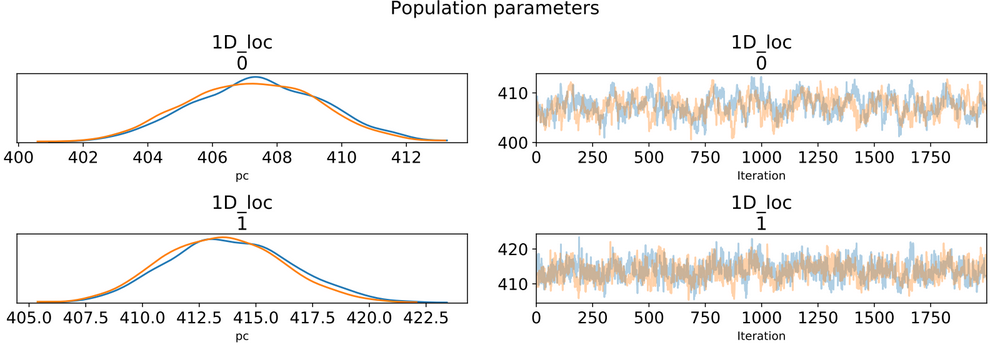
\includegraphics[width= 0.8\textwidth]{gmm_ngc1662cut.png}
\caption{\label{fig:gmm_ngc1662cut} Resultados dos parâmetros do aglomerado para a amostra \(A_{cut}\) para o prior GMM}
\end{figure}

Outro resultado interessante foi obtido quando avaliado o prior Uniforme (Figura \ref{fig:uniforme_ngc1662}). Apesar de apresentar distribuições de probabilidade com pico estreito e bem definido para o aglomerado, este método também provocou uma distribuição ampla e achatada para as estrelas individuais. Esta discrepância é explicada justamente pelo fato deste ser o prior menos informativo de todos, não impondo uma tendência de agrupamento forte no centro. Isso permite que as estrelas se distribuam igualmente ao longo do aglomerado, apresentando uma incerteza individual grande. Por outro lado, esta distribuição não se repete quando estudado o aglomerado como um todo, pois o conjunto de 384 estrelas proporciona uma verossimilhança forte e os erros aleatórios de cada estrela são anulados, proporcionando uma distribuição de pico bem definido.

\begin{figure}[ht]
\centering
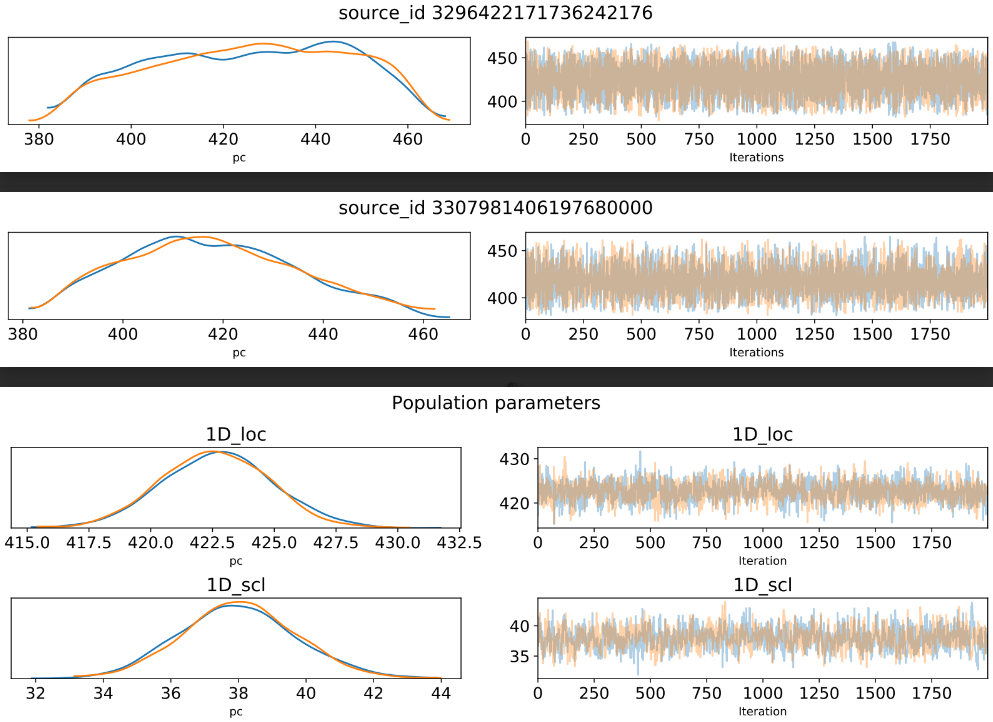
\includegraphics[width= 0.8\textwidth]{uniforme_ngc1662.png}
\caption{\label{fig:uniforme_ngc1662} Resultados da amostra \(A_{full}\) para o prior Uniforme}
\end{figure}

Comparando-se os resultados da amostra \(A_{full}\), nota-se que houve similaridade considerável entre os resultados, de modo que tanto as distribuições de probabilidade (Figura \ref{fig:ngc1662_comparison}) quanto os valores de distâncias calculadas para cada prior foram semelhantes. Com exceção do caso GMM, também aparentou haver semelhança quando equiparadas as amostras \(A_{full}\) e \(A_{cut}\). Para confirmar se os priors destas amostras eram de fato compatíveis, foi realizado um Teste-Z com intervalo de confiança \(2\sigma\), de maneira que verificou-se que apenas o prior Uniforme não foi estatisticamente compatível (Tabela \ref{tab:zscore_estabilidade_final}), evidenciando sua sensibilidade extrema a possíveis outliers.

É importante notar que, embora os Testes-Z calculados assumam a independência entre as amostras, isso é uma simplificação conservadora. Dado que a amostra selecionada é um subconjunto da amostra completa, as distâncias são positivamente correlacionadas. A inclusão do termo de covariância apenas aumentaria o valor de Z para todos os priors, reforçando ainda mais a incompatibilidade estatística do Prior Uniforme, enquanto para os outros esse acréscimo provavelmente não seria tão relevante, devido aos já muito baixos valores de Teste-Z obtidos nestes casos.

\begin{figure}[ht]
\centering
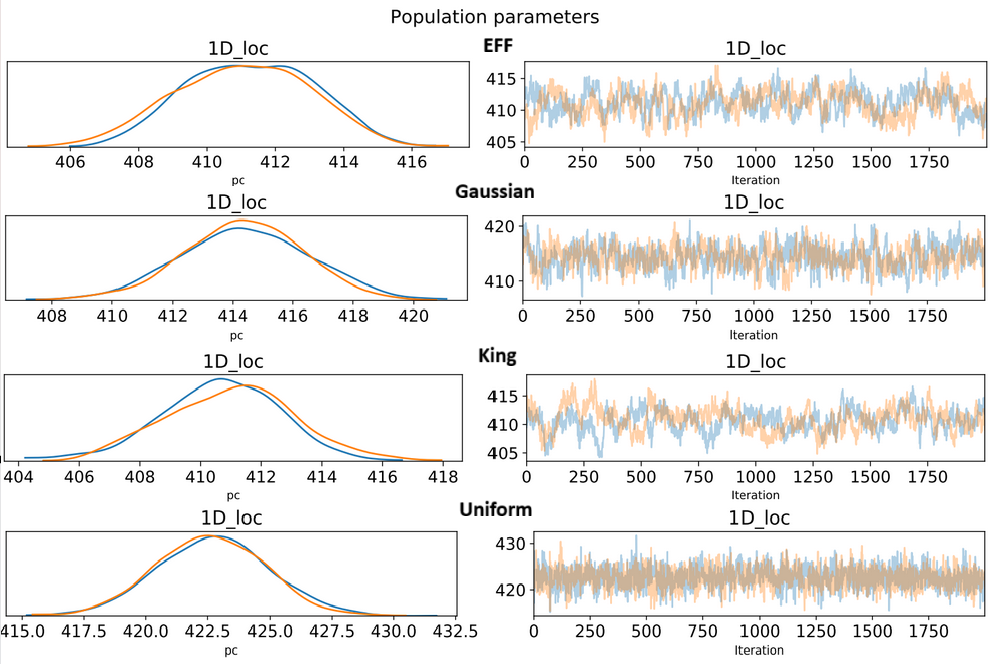
\includegraphics[width= 0.8\textwidth]{ngc1662_comparison.png}
\caption{\label{fig:ngc1662_comparison} Resultados da amostra \(A_{full}\) para os priors EFF, Gaussiano, King e Uniforme.}
\end{figure}

\begin{table}[h]
    \centering
    \caption{Análise de Estabilidade (Teste-Z): Compatibilidade das Distâncias entre as Amostras $A_{\text{full}}$ e $A_{\text{cut}}$ para os 4 diferentes priors analisados.}
    \label{tab:zscore_estabilidade_final}
    \renewcommand{\arraystretch}{1.5} % Aumenta o espaçamento vertical para clareza
    \begin{tabular}{|l|>{\centering}m{2.5cm}|>{\centering}m{2.5cm}|>{\centering}m{1.5cm}|>{\centering\arraybackslash}m{2.5cm}|}
        \hline
        \textbf{Prior} & $\mathbf{A_{\text{full}}} [pc]$ & $\mathbf{A_{\text{cut}}}$ [pc] & \textbf{Teste-Z} & \textbf{Compatíveis ($Z < 2$)} \\
        \hline
        EFF  & $410,9^{+1,9}_{-\text{1,7}}$ & $410,1^{+2,1}_{-\text{2,05}}$ & $0,28$ & Sim \\
        \hline
        Gaussiano & $414,1^{+2,1}_{-\text{2,0}}$ & $411,4^{+2,0}_{-\text{2,0}}$ & $0,95$ & Sim \\
        \hline
        King & $410,9^{+2,0}_{-\text{2,2}}$ & $409,9^{+2,0}_{-\text{2,2}}$ & $0,34$ & Sim \\
        \hline
        Uniforme & $422,6^{+2,2}_{-\text{2,1}}$ & $413,8^{+2,0}_{-\text{1,9}}$ & $\mathbf{3,06}$ & \textbf{Não} \\
        \hline
    \end{tabular}
    \renewcommand{\arraystretch}{1.0} % Retorna ao padrão
\end{table}

Analisada a compatibilidade entre amostras, o último passo foi a comparação entre resultados do Kalkayotl com estimativas de distância da literatura. Dado que três dos quatro priors se mostraram compatíveis amostralmente, utilizou-se apenas a amostra selecionada \(A_{cut}\) para esta etapa. Devido à ausência de incertezas nos resultados fornecidos por \cite{cantat-gaudin_painting_2020} e \cite{dias_new_2002}, estes foram comparados apenas de maneira quantitativa aos resultados do Kalkayotl, de modo que o primeiro se mostrou muito próximo do obtido, enquanto o segundo apresentou uma disparidade grande, justificada pela imprecisão das medidas efetuadas pelo Hipparcus quando comparado ao Gaia e à utilização do método da inversão da paralaxe. Com relação às estimativas de \cite{dias_updated_2021} e \cite{hunt_improving_2024}, foi realizado novamente o Teste-Z para um intervalo de confiança de \(2\sigma\) (Tabela \ref{tab:comparacao_final}).

\begin{table}[h]
    \centering
    \caption{Comparação Final dos Priors com a amostra selecionada ($A_{\text{cut}}$) e Teste-Z (\(2\sigma\)) com os valores da literatura.}
    \label{tab:comparacao_final}
    \renewcommand{\arraystretch}{1.5} % Aumenta o espaçamento vertical
    \begin{tabular}{|l|c|c|c|c|c|}
        \hline
        \textbf{Prior} & $\mathbf{A_{\text{cut}}}$ [pc] & $\mathbf{Z_{\text{Dias-A}_{\text{cut}}}}$ & \textbf{Comp. Dias} & $\mathbf{Z_{\text{Hunt-A}_{\text{cut}}}}$ & \textbf{Comp. Hunt} \\
        \hline
        EFF & $410,10^{+2,05}_{-\text{2,05}}$ & $0,03$ & Sim & $2,66$ & \textbf{Não} \\
        \hline
        Gaussiano & $411,40^{+1,95}_{-\text{2,00}}$ & $0,39$ & Sim & $3,40$ & \textbf{Não} \\
        \hline
        King & $409,90^{+1,95}_{-\text{2,15}}$ & $0,03$ & Sim & $2,56$ & \textbf{Não} \\
        \hline
        Uniforme & $413,80^{+2,00}_{-\text{1,90}}$ & $1,06$ & Sim & $4,67$ & \textbf{Não} \\
        \hline
    \end{tabular}
    \renewcommand{\arraystretch}{1.0} % Retorna ao padrão
\end{table}

Nota-se que houve compatibilidade de todos os priors com o catálogo de \cite{dias_updated_2021}, enquanto que \cite{hunt_improving_2024} não concordou com nenhum dos valores obtidos. Essa divergência pode estar associada ao valor baixo da incerteza obtida por Hunt, podendo esta estar subestimada.

Conclui-se por meio deste projeto que os priors mais úteis para o estudo da distância do aglomerado NGC 1662 foram EFF, Gaussiano e King, dado que todos apresentaram distribuição de probabilidade bem definida e suas cadeias de Markov convergiram para valores estáveis. Além disso, todos se mostraram compatíveis quando comparadas entre si as amostras \(A_{full}\) e \(A_{cut}\), bem como quando equiparados ao catálogo de \cite{dias_updated_2021}, mostrando resultados sólidos. Portanto, dada a robustez interna, os priors EFF, Gaussiano e King são os mais úteis para a determinação das distâncias de aglomerados próximos (\(<500pc\)) e bem populados (\(>200\) membros). Devido à sua simplicidade e acurácia, o prior Gaussiano e sua estimativa de distância de $411,4^{+2,0}_{-\text{2,0}}$ foram adotados pelo autor deste projeto como os mais úteis para a ocasião. Os resultados obtidos por estas famílias são estatisticamente compatíveis com a estimativa de ajuste de isócronas de Dias et al. (\citeyear{dias_updated_2021}), demonstrando a consistência do método Kalkayotl com a literatura do Gaia DR2.

\section{Conclusão}

A determinação precisa de distâncias de aglomerados estelares é um dos pilares da Astronomia Galáctica, sendo fundamental para calibrar a Escala de Distância Cósmica. O desafio de obter incertezas robustas, especialmente por conta das sistemáticas como a correlação espacial das paralaxes, foi o ponto central deste projeto. Para superar isso, empregamos o framework inovador de Inferência Bayesiana hierárquica do código Kalkayotl \cite{olivares_kalkayotl_2020}.

Aplicado a diferentes tipos de priors, Kalkayotl se mostrou preciso para o aglomerado NGC 1662, tanto em sua amostra completa \(A_{full}\) quanto na selecionada \(A_{cut}\), proporcionando medidas robustas de distribuição de probabilidade de distâncias e iterações MCMC, de modo que, por meio da análise dos resultados, foi possível determinar a qualidade de cada prior na realização desta tarefa.

Foi evidenciado que, para amostras ruidosas, sem seleção, o prior GMM resulta em estimativas ruins de distância, visto que acaba sendo contaminado por outliers. Entretanto, quando aplicado a amostras filtradas, apresenta bom desempenho, entregando resultados similares a valores da literatura. Dado que este valor não possuía contrapartida na amostra completa, foi decidido não utilizar a estimativa de distância de \(A_{cut}\) nas outras análises do projeto.

Notou-se também que o prior Uniforme apresenta uma distribuição muito esparsa dos valores de distância de estrelas individuais, visto que assume uma distribui-se equivalentemente em todos os pontos do aglomerado, porém desempenha bem quando considerada a distância do aglomerado como um todo, visto que as incertezas aleatórias do alto número de membros acabam se cancelando e proporcionando uma distribuição mais bem definida.

Quando estudadas as duas amostras, verificou-se compatibilidade para um intervalo de confiança de \(2\sigma\) para os priors EFF, Gaussiano e King, mostrando fortes argumentos sobre a estrutura mais simples de NGC 1662, enquanto o Uniforme se mostrou incompatível, enfatizando sua alta sensibilidade a conjuntos de dados ruidosos.

Por fim, na comparação com a literatura, resultados de teste-Z para a amostra \(A_{cut}\) mostraram compatibilidade com os resultados catalogados por \cite{dias_updated_2021}, porém não concordaram com a distância de NGC 1662 fornecida por \cite{hunt_improving_2024}, divergência que pode estar atrelada a incertezas subestimadas pela autora deste catálogo.


Portanto, os priors estáveis são os mais adequados para o estudo de aglomerados próximos. O resultado final do Kalkayotl, utilizando o prior Gaussiano da amostra selecionada, forneceu a distância de  $411,4^{+2,0}_{-\text{2,0}}$ parsecs, sendo este o prior considerado o mais útil para os fins deste projeto.

% No seu arquivo main.tex:
% ... SEU DOCUMENTO TERMINA AQUI ...


\bibliography{bibtex} % Apenas o comando para carregar os dados
%\begin{thebibliography}{99}
%\end{thebibliography}

\end{document}


